\chapter{Shift register}

\section{Shift register}
\paragraph{Traccia}
Progettare, implementare in VHDL e testare mediante simulazione un registro a scorrimento di N bit in grado di shiftare a destra o a sinistra di un numero Y variabile di posizioni a seconda di una opportuna selezione. Il componente deve essere realizzato utilizzando sia un a) approccio comportamentale sia un b) approccio strutturale.  
Nota: il numero di bit del registro X e i valori che può assumere il parametro Y possono essere scelti dallo studente (ad es. X=8 e Y= {1,2}).

\section{Soluzione Comportamentale}
\subsection{Architettura}
Per l'implementazione della soluzione è stato implementato un sistema che riceve i seguenti segnali di ingresso:
\begin{itemize}
\item \textit{input} è un vettore di 2 bit, che rappresenta gli ingressi che vengono inseriti nel registro;
\item \textit{clock} è il segnale per la tempificazione;
\item \textit{reset} è un segnale per resettare la macchina e farla partire da uno stato noto;
\item \textit{direction} indica il verso di shift, nel programma è stato assunto come ipotesi che il valore direction=0 indichi uno shift verso destra e direction=1 indichi uno shift verso sinistra;
\item \textit{y} è la variabile che indica il numero di shift che è possibile effettuare, in particolare è stato definito come Y=0 lo shift di un solo bit per volta e Y=1 lo shift di due bit per volta;
\end{itemize}

Il sistema presenta il seguente segnale di uscita:
\begin{itemize}
\item \textit{output} è un vettore di 4 bit che rappresenta i valori contenuti nei singoli registri.
\end{itemize}

 È previsto che l'utente debba inserire due bit per controllare il dispositivo, un bit per selezionare il verso di shift e un bit per selezionare il numero di shift. Per ipotesi si assume che nel caso di y=0 (1 solo shift) il comportamento dello shift register è di tipo SIPO (Single Input Parallel Output), mentre per y=1 (2 shift per volta) si assume che il comportamento dello shift regiser è di tipo PIPO (Parallel Input Parallel Output). Per realizzare queste distinzioni di comportamento sono state definite diverse selezioni, al cui intero avviene propagazione dei bit tramite i segnali s1,s2,s3 e s4. Il reset è stato realizzato in modalità sincrona.
 
 Data la possibilità che il sistema scorra di due posizioni è stato deciso di predisporre un ingresso dati di due bit. Durante la modalità y=0 a un solo shift viene letto solo il bit meno significativo, che viene inserito in s1, mentre con y=1 vengono letti entrambi, e vengono inseriti in s1 e s2. Senza questa modifica all'input, nel caso dello shift doppio, si avrebbe una duplicazione del dato. È però importante prendere solo un bit durante lo shift singolo, altrimenti si avrebbe un problema si sovrascrizione come mostrato in Figura \ref{fig:errore}.
 
\begin{figure}[H]
    \centering
    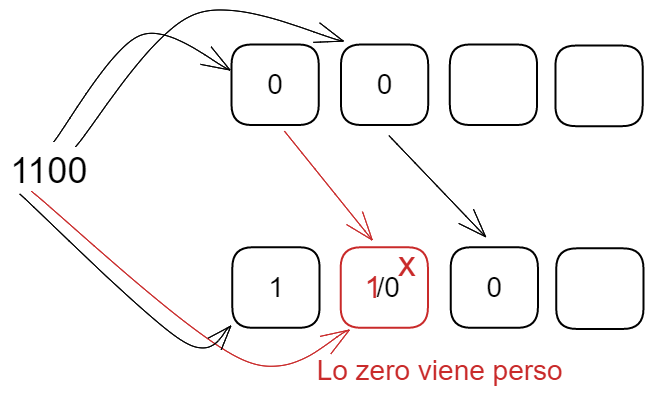
\includegraphics[width=11cm]{immagini/esercizio4/errore.png}
    \caption{Errore}
    \label{fig:errore}
\end{figure}
 
 
La realizzazione tramite approccio comportamentale è stata implementata mediante il seguente codice:
\begin{lstlisting} [language=VHDL, caption=Shift register (Behavioural)]
library IEEE;
use IEEE.STD_LOGIC_1164.ALL;

entity shift_reg_behavioural is
    Port (
        input: in std_logic_vector (1 downto 0);
        clock: in std_logic ;
        reset: in std_logic ;
        direction: in std_logic ; -- 0 shifta a destra, 1 shifta a sinistra
        y: in std_logic; --se Y=0 shift da 1, se Y=1 shift da 2
        output: out std_logic_vector (3 downto 0)
    );
end shift_reg_behavioural;

architecture Behavioral of shift_reg_behavioural is
    signal s1,s2,s3,s4 : std_logic;
begin
    process (clock)
    begin
        if (rising_edge (clock)) then
            if ( reset='1') then
                s1<='0';
                s2<='0';
                s3<='0';
                s4<='0';
            else
                if(y='0') then
                    if(direction ='0') then
                        --destra
                        s1<=input(0) ;
                        s2<=s1;
                        s3<=s2;
                        s4<=s3;

                    elsif (direction ='1') then
                        --sinistra
                        s4<=input(0) ;
                        s3<=s4;
                        s2<=s3;
                        s1<=s2;
                    end if;

                elsif (y='1') then
                    if(direction ='0') then
                        --destra
                        s1<=input(1);
                        s2<=input(0);
                        s3<=s1;
                        s4<=s2;

                    elsif (direction ='1') then
                        --sinistra
                        s4<=input(1);
                        s3<=input(0);
                        s2<=s4;
                        s1<=s3;
                    end if;
                end if;
           end if;
        end if;
    end process;

output<= s1 & s2 & s3 & s4;

end Behavioral;
\end{lstlisting}

\subsection{Simulazione}
In primo luogo è stata effettuata una wait di 100 ns per aspettare che il segnale di GRS (Global Set Reset) diventasse alto ed è stata resettata la macchina. Sono stati effettuati quattro casi di test.
I primi due sono stati verificati sfruttando gli stessi input, impostando Y=0 (effettuando uno shift per volta), facendo variare unicamente la direzione da 0 a 1 (da destra a sinistra).
In modo duale sono stati verificati gli altri due casi di test, impostando Y=1 (effettuando due shift per volta).

\paragraph{Testbench}

\begin{lstlisting} [language=VHDL, caption=Testbench a example]
library IEEE;
use IEEE.STD_LOGIC_1164.ALL;

entity shift_ref_behavioural_TB is
end shift_ref_behavioural_TB;

architecture Behavioral of shift_ref_behavioural_TB is

    component shift_reg_behavioural is
        Port (
            input: in std_logic_vector (1 downto 0);
            clock: in std_logic ;
            reset: in std_logic ;
            direction: in std_logic ; -- 0 shifta a destra, 1 shifta a sinistra
            y: in std_logic; --se Y=0 shift da 1, se Y=1 shift da 2
            output: out std_logic_vector (3 downto 0)
        );

    end component  shift_reg_behavioural;

  signal s_input: std_logic_vector (1 downto 0):=(others => '0');
  signal s_output: std_logic_vector (3 downto 0):=(others => '0');
  signal s_clock, s_reset, s_direction,s_y: std_logic := '0';
  constant clk_period: time := 10 ns;

begin
    uut: shift_reg_behavioural
        port map(
            input=>s_input ,
            output=>s_output,
            clock=>s_clock,
            reset=>s_reset,
            direction=>s_direction,
            y=>s_y
        );

    clock: process
    begin
        s_clock <= '1';
        wait for clk_period/2;
        s_clock <= '0';
        wait for clk_period/2;
    end process clock;

    TB: process
    begin
        wait for 100ns;
        s_reset <='1';
        wait for clk_period;
        s_reset <='0';

        -- Caso di test 1 (Y=0, direction=0)
        s_y <='0';
        s_input<="01";
        wait for clk_period;
        assert (s_output = "1000") report "ERRORE";

        s_input<="00";
        wait for clk_period;
        assert (s_output = "0100") report "ERRORE";

        s_input<="00";
        wait for clk_period;
        assert (s_output = "0010") report "ERRORE";

        s_input<="01";
        wait for clk_period;
        assert (s_output = "1001") report "ERRORE";

        -- Caso di test 2 (Y=0, direction=1)
        s_y <='0';
        s_direction <='1';
        s_reset<='1';
        wait for clk_period;
        s_reset<='0';

        s_input<="01";
        wait for clk_period;
        assert (s_output = "0001") report "ERRORE";

        s_input<="00";
        wait for clk_period;
        assert (s_output = "0010") report "ERRORE";

        s_input<="00";
        wait for clk_period;
        assert (s_output = "0100") report "ERRORE";

        s_input<="01";
        wait for clk_period;
        assert (s_output = "1001") report "ERRORE";

        -- Caso di test 1 (Y=1, direction=0)
        s_y <='1';
        s_direction <='0';
        s_reset<='1';
        wait for clk_period;
        s_reset<='0';

        s_input<="11";
        wait for clk_period;
        assert (s_output = "1100") report "ERRORE";

        s_input<="00";
        wait for clk_period;
        assert (s_output = "0011") report "ERRORE";

        s_input<="11";
        wait for clk_period;
        assert (s_output = "1100") report "ERRORE";

        s_input<="01";
        wait for clk_period;
        assert (s_output = "0111") report "ERRORE";

        -- Caso di test 4 (Y=1, direction=1)
        s_y <='1';
        s_direction <='1';
        s_reset<='1';
        wait for clk_period;
        s_reset<='0';

        s_input<="11";
        wait for clk_period;
        assert (s_output = "0011") report "ERRORE";

        s_input<="00";
        wait for clk_period;
        assert (s_output = "1100") report "ERRORE";

        s_input<="11";
        wait for clk_period;
        assert (s_output = "0011") report "ERRORE";

        s_input<="01";
        wait for clk_period;
        assert (s_output = "1110") report "ERRORE";

        wait;
    end process;
end Behavioral;
\end{lstlisting}


\begin{figure}[H]
    \centering
    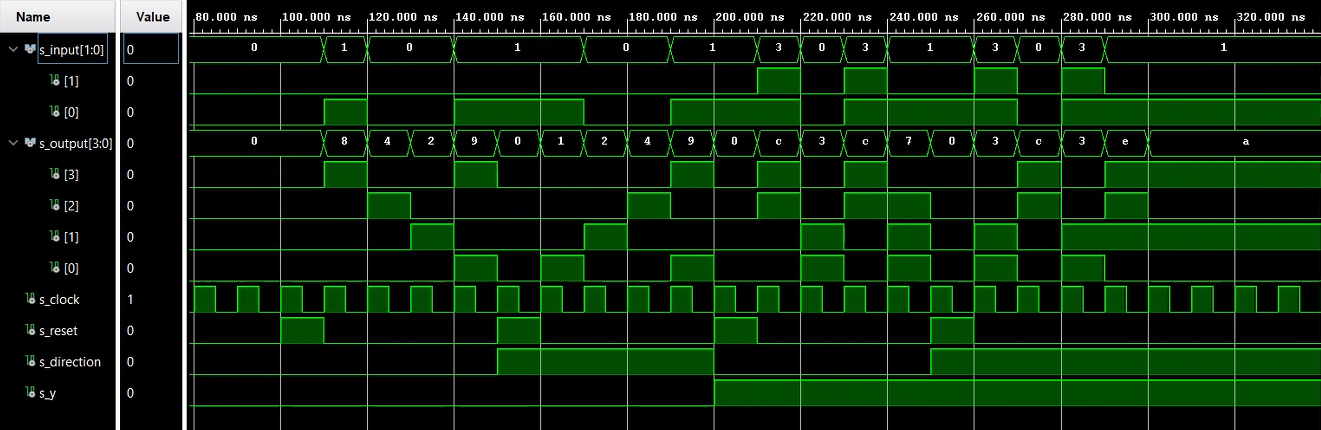
\includegraphics[width=16cm]{immagini/esercizio4/output_simulazione_4.1.png}
    \caption{Output della simulazione}
    \label{fig:notebook}
\end{figure}

\section{Soluzione Strutturale}
\subsection{Architettura}
Il sistema è stato realizzato seguendo un approccio strutturale. In primo luogo sono stati realizzati dei flip flop edge triggered da 1 bit con un semplice processo. Data la complessità dei comandi disponibili dall'utente, si è scelto di realizzare una rete di controllo che gestisce i flip flop e la comunicazione tra essi. Sarebbe stato possibile anche mappare gli input di controllo a una serie di multiplexer in modo da non utilizzare processi, e rendere il sistema più scalabile, ma date le dimensioni ridotte richieste si è scelto un compromesso tra performance e complessità.
La rete di controllo prende in input le uscite dei registri e le smista , tramite il suo output, alle entrate degli stessi, cambiando i flussi dei dati a seconda della modalità. Per fare ciò vengono utilizzati 8 segnali. 
È da notare che mentre i flip flop si attivano sul fronte di discesa del clock, la rete di controllo lo fa su quello di salita. In questo modo, in un singolo colpo di clock, entrambi i componenti possono funzionare senza la creazione di delay causati dall'invio e dalla ricezione dei segnali. In entrambi i componenti si è utilizzato un reset sincrono.

L'architettura si presenta come segue:
\begin{figure}[H]
    \centering
    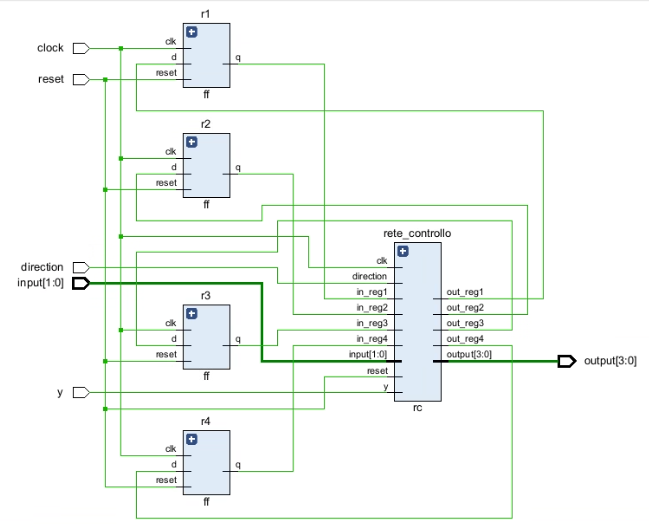
\includegraphics[width=17cm]{immagini/esercizio4/schema_4.2.png}
    \caption{Schema architettura}
    \label{fig:notebook}
\end{figure}

Il componente flip flop è stato realizzato mediante il seguente codice:

\begin{lstlisting}[language=VHDL, caption=flip flop]
library IEEE;
use IEEE.STD_LOGIC_1164.ALL;

entity ff is
    Port (
        d, clk, reset: in std_logic ;
        q: out std_logic );
end ff;
architecture Behavioral of ff is
begin
    process (clk)
    begin
        if falling_edge(clk) then
            if (reset='1') then
                q<='0';
            else
                q<=d;
            end if;
        end if;
    end process;
end Behavioral;
\end{lstlisting}

La rete di controllo è stata realizzata mediante il seguente codice:

\begin{lstlisting}[language=VHDL, caption=Rete di controllo]
library IEEE;
use IEEE.STD_LOGIC_1164.ALL;

entity rc is
    Port (
        input: in std_logic_vector (1 downto 0);
        clk, reset , direction , y: in std_logic ;
        in_reg1, in_reg2, in_reg3, in_reg4: in std_logic;
        out_reg1,out_reg2,out_reg3, out_reg4:out std_logic;
        output: out std_logic_vector (3 downto 0)
    );
end rc;

architecture Behavioral of rc is

begin
    process (clk)
    begin
        if (rising_edge (clk)) then
            if ( reset='1') then
                out_reg1 <='0';
                out_reg2 <='0';
                out_reg3 <='0';
                out_reg4 <='0';

            else
                if(y='0') then
                    if(direction ='0') then
                        --destra
                        out_reg1<=input(0);
                        out_reg2<=in_reg1;
                        out_reg3<=in_reg2;
                        out_reg4<=in_reg3;

                    elsif (direction ='1') then
                        --sinitra
                        out_reg4<=input(0) ;
                        out_reg3<=in_reg4;
                        out_reg2<=in_reg3;
                        out_reg1<=in_reg2;
                    end if;

                elsif (y='1') then
                    if(direction ='0') then
                        --destra
                        out_reg1<=input(1);
                        out_reg2<=input(0);
                        out_reg3<=in_reg1;
                        out_reg4<=in_reg2;

                    elsif (direction ='1') then
                        --sinitra
                        out_reg4<=input(1);
                        out_reg3<=input(0);
                        out_reg2<=in_reg4;
                        out_reg1<=in_reg3;
                    end if;
                end if;
            end if;
        end if;
    end process;
    
    output<=in_reg1 & in_reg2 & in_reg3 & in_reg4;

end Behavioral;
\end{lstlisting}

Lo shift register è stato generato tramite il collegamento degli opportuni componenti: 4 flip-flop e 1 rete di controllo:
\begin{lstlisting} [language=VHDL, caption=Shift Register (Structural)]
library IEEE;
use IEEE.STD_LOGIC_1164.ALL;

entity shift_register is
    Port (
        input: in std_logic_vector (1 downto 0);
        clock: in std_logic ;
        reset: in std_logic ;
        direction: in std_logic ; -- 0 shifta a destra, 1 shifta a sinistra
        y: in std_logic; --se Y=0 shift da 1, se Y=1 shift da 2
        output: out std_logic_vector (3 downto 0)
    );
end shift_register;

architecture Structural of shift_register is

    component ff is port (
        d, clk, reset: in std_logic ;
        q: out std_logic 
     );
    end component ff;

    component  rc is port (
          input: in std_logic_vector (1 downto 0);
          clk, reset , direction , y: in std_logic ;
          in_reg1, in_reg2, in_reg3, in_reg4: in std_logic;
          out_reg1,out_reg2,out_reg3, out_reg4:out std_logic;
          output: out std_logic_vector (3 downto 0)
        );
    end component rc;

    signal s_in_reg1,  s_in_reg2,  s_in_reg3,  s_in_reg4 : std_logic:='0';
    signal s_out_reg1, s_out_reg2, s_out_reg3,  s_out_reg4: std_logic:='0';
    signal s_output: std_logic_vector (3 downto 0);

begin

    r1: ff  port map(
            d=>s_out_reg1,
            clk=> clock,
            reset=> reset,
            q => s_in_reg1 );

    r2: ff  port map(
            d=>s_out_reg2,
            clk=> clock,
            reset=> reset,
            q => s_in_reg2 );

    r3: ff  port map(
            d=>s_out_reg3,
            clk=> clock,
            reset=> reset,
            q => s_in_reg3 );

    r4: ff  port map(
            d=>s_out_reg4,
            clk=> clock,
            reset=> reset,
            q => s_in_reg4 );

    rete_controllo: rc  port map(
            input=> input,
            clk=> clock,
            reset=> reset,
            direction=> direction,
            y=> y,
            in_reg1=> s_in_reg1,
            in_reg2=> s_in_reg2,
            in_reg3=> s_in_reg3,
            in_reg4=> s_in_reg4,

            out_reg1=> s_out_reg1,
            out_reg2=> s_out_reg2,
            out_reg3=> s_out_reg3,
            out_reg4=> s_out_reg4,
            output=>s_output );
        
        output<=s_output;
        
end Structural;
\end{lstlisting}

\subsection{Simulazione}
Il testing di questa rete è stato effettuato con lo stesso testbench che è stato utilizzato nell'approccio comportamentale, che quindi per semplicità viene omesso, avendo dichiarato volutamente gli stessi input e output dell'intera rete. È stato possibile confrontare i due risultati e constatare il corretto funzionamento di entrambi. 

L'output che deriva dal testbench è il seguente:
\begin{figure}[H]
    \centering
    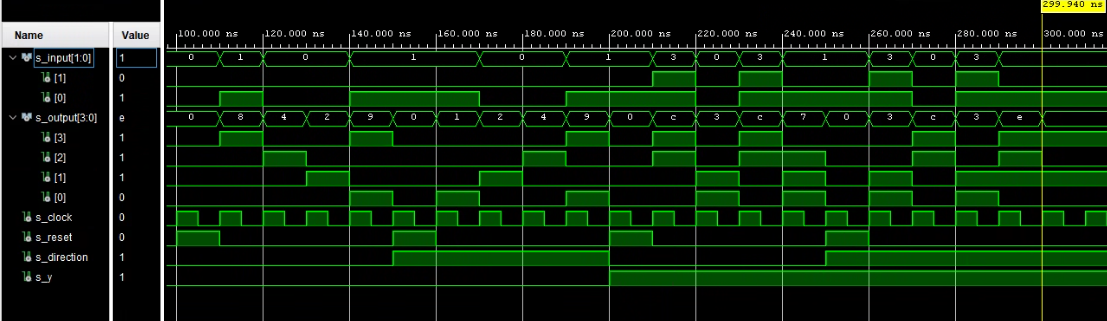
\includegraphics[width=16cm]{immagini/esercizio4/output_simulazione_4.2.png}
    \caption{Output della simulazione}
    \label{fig:notebook}
\end{figure}